\documentclass{ctexart}
\usepackage{graphicx} % Required for inserting images
\usepackage{amsmath}
\usepackage{booktabs}
\usepackage[left=2.5cm,right=2.5cm,top=2.5cm,bottom=2.5cm]{geometry}
\begin{document}
\section{实验目的}
\begin{enumerate}
    \item 研究一阶RC电路的方波响应;
    \item 测量一阶电路的时间常数;
    \item 实现微分和积分电路;
\end{enumerate}
\section{实验原理}
\subsection{确定实验内容1的电路电阻取值}
实验1要求时间常数$\tau$=0.066ms。根据公式
\begin{equation}
    \tau=RC
\end{equation}
可得电阻取值为
\begin{equation}
    R=\dfrac{\tau}{C}=3k\Omega
\end{equation}
\subsection{按照实验2参数要求,结合自身已有元件参数,设计微分、积分电路。并用Multisim进行仿真,预先测量记录相应的波形及数据}
\subsubsection{积分电路}
设计如图\ref{fig:积分电路}所示的RC电路。设置电源电压幅值$U_S=5V$,频率为$f=22727Hz$,电阻为$R=10k\Omega$,电容为$C=22nF$。
\begin{figure}[!ht]
    \centering
    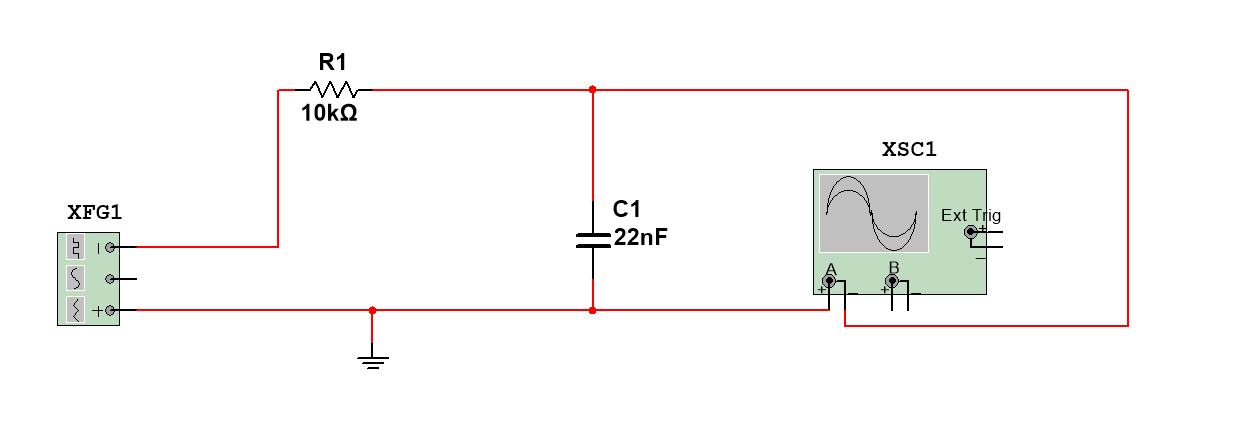
\includegraphics[scale=0.5]{pic/积分电路.png}
    \caption{积分电路}
    \label{fig:积分电路}
\end{figure}
通过示波器显示如图\ref{fig:示波器1}所示的波形,得到其最大值为123.501mV,最小值为-123.687mV。
\begin{figure}
    \centering
    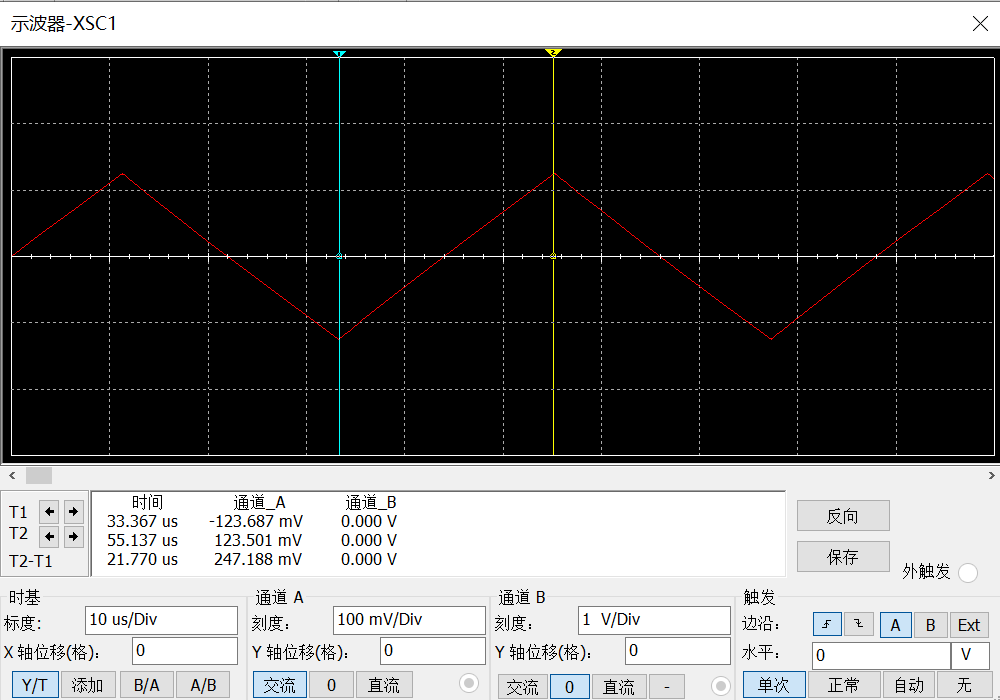
\includegraphics[scale=0.8]{pic/示波器1.png}
    \caption{示波器1}
    \label{fig:示波器1}
\end{figure}
已知电容的特性为
\begin{equation}
    U_C=\dfrac{1}{C}\int_0^t i(t)dt
\end{equation}
又由于时间常数$\tau$远大于5倍周期,因此在电容电压的每个波形内,电容都没有充分充放电,将输入电压的方波近似为了锯齿波,电阻上的电压占总电压的绝大部分。因此有
\begin{equation}
    U_C=\dfrac{1}{C}\int_0^t i(t)dt =\dfrac{1}{RC}\int _0^t U_s(t)dt
\end{equation}
输出电压的极差
\begin{equation}
    \Delta U_O = 247.188mV 
\end{equation}
\begin{equation}
    \dfrac{\Delta U_O}{U_S}=0.049
\end{equation}
\subsection{微分电路}
\begin{figure}
    \centering
    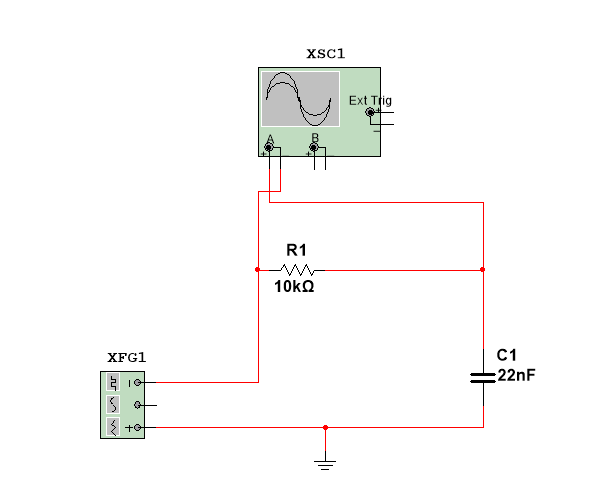
\includegraphics{pic/微分电路.png}
    \caption{微分电路}
    \label{fig:微分电路}
\end{figure}
保持上一步的电路结构,将示波器接到电阻两端,并将电源频率设置为100Hz,此时$\tau$远小于周期T,故在绝大部分时间内$U_C=U_S$,
继而有
\begin{equation}
    U_O(t)=Ri(t)=RC\dfrac{dU_C(t)}{dt}=RC\dfrac{dU_S(t)}{dt}
\end{equation}
\begin{figure}
    \centering
    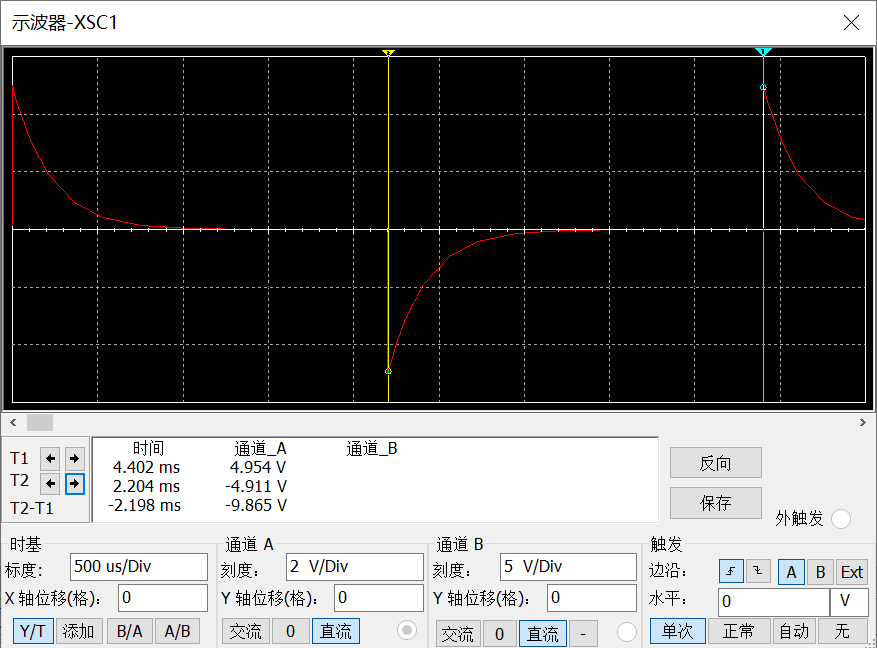
\includegraphics{pic/示波器2.png}
    \caption{示波器2}
    \label{fig:示波器2}
\end{figure}
输出电压的峰峰值
\begin{equation}
    \Delta U_O = 9.865V 
\end{equation}
\begin{equation}
    \dfrac{\Delta U_O}{U_S}=1.973
\end{equation}
因此,只需要测量输出电压再除以时间常数即可求得电压源函数关于时间的微分。但需要注意的是,该等式仅在大约0.1T时间内有效(即图中波形不为零的部分)且计算精度波动较大。
\section{实验内容}
\subsection{研究RC电路的方波响应}
\subsubsection{激励信号取频率为 1kHz,高电平电压为 5V,低电平电压为 0V 的方波。用示波器观察测量并记录方波响应的波形,解释观察到的波形现象。}
经过实验原理部分的计算,我们得到:电阻应当选取$R=3k\Omega$,设计电路图如图!!!所示。测量得到的$u_C(t)$信号波形为图\ref{fig:1-1}所示
\begin{figure}
    \centering
    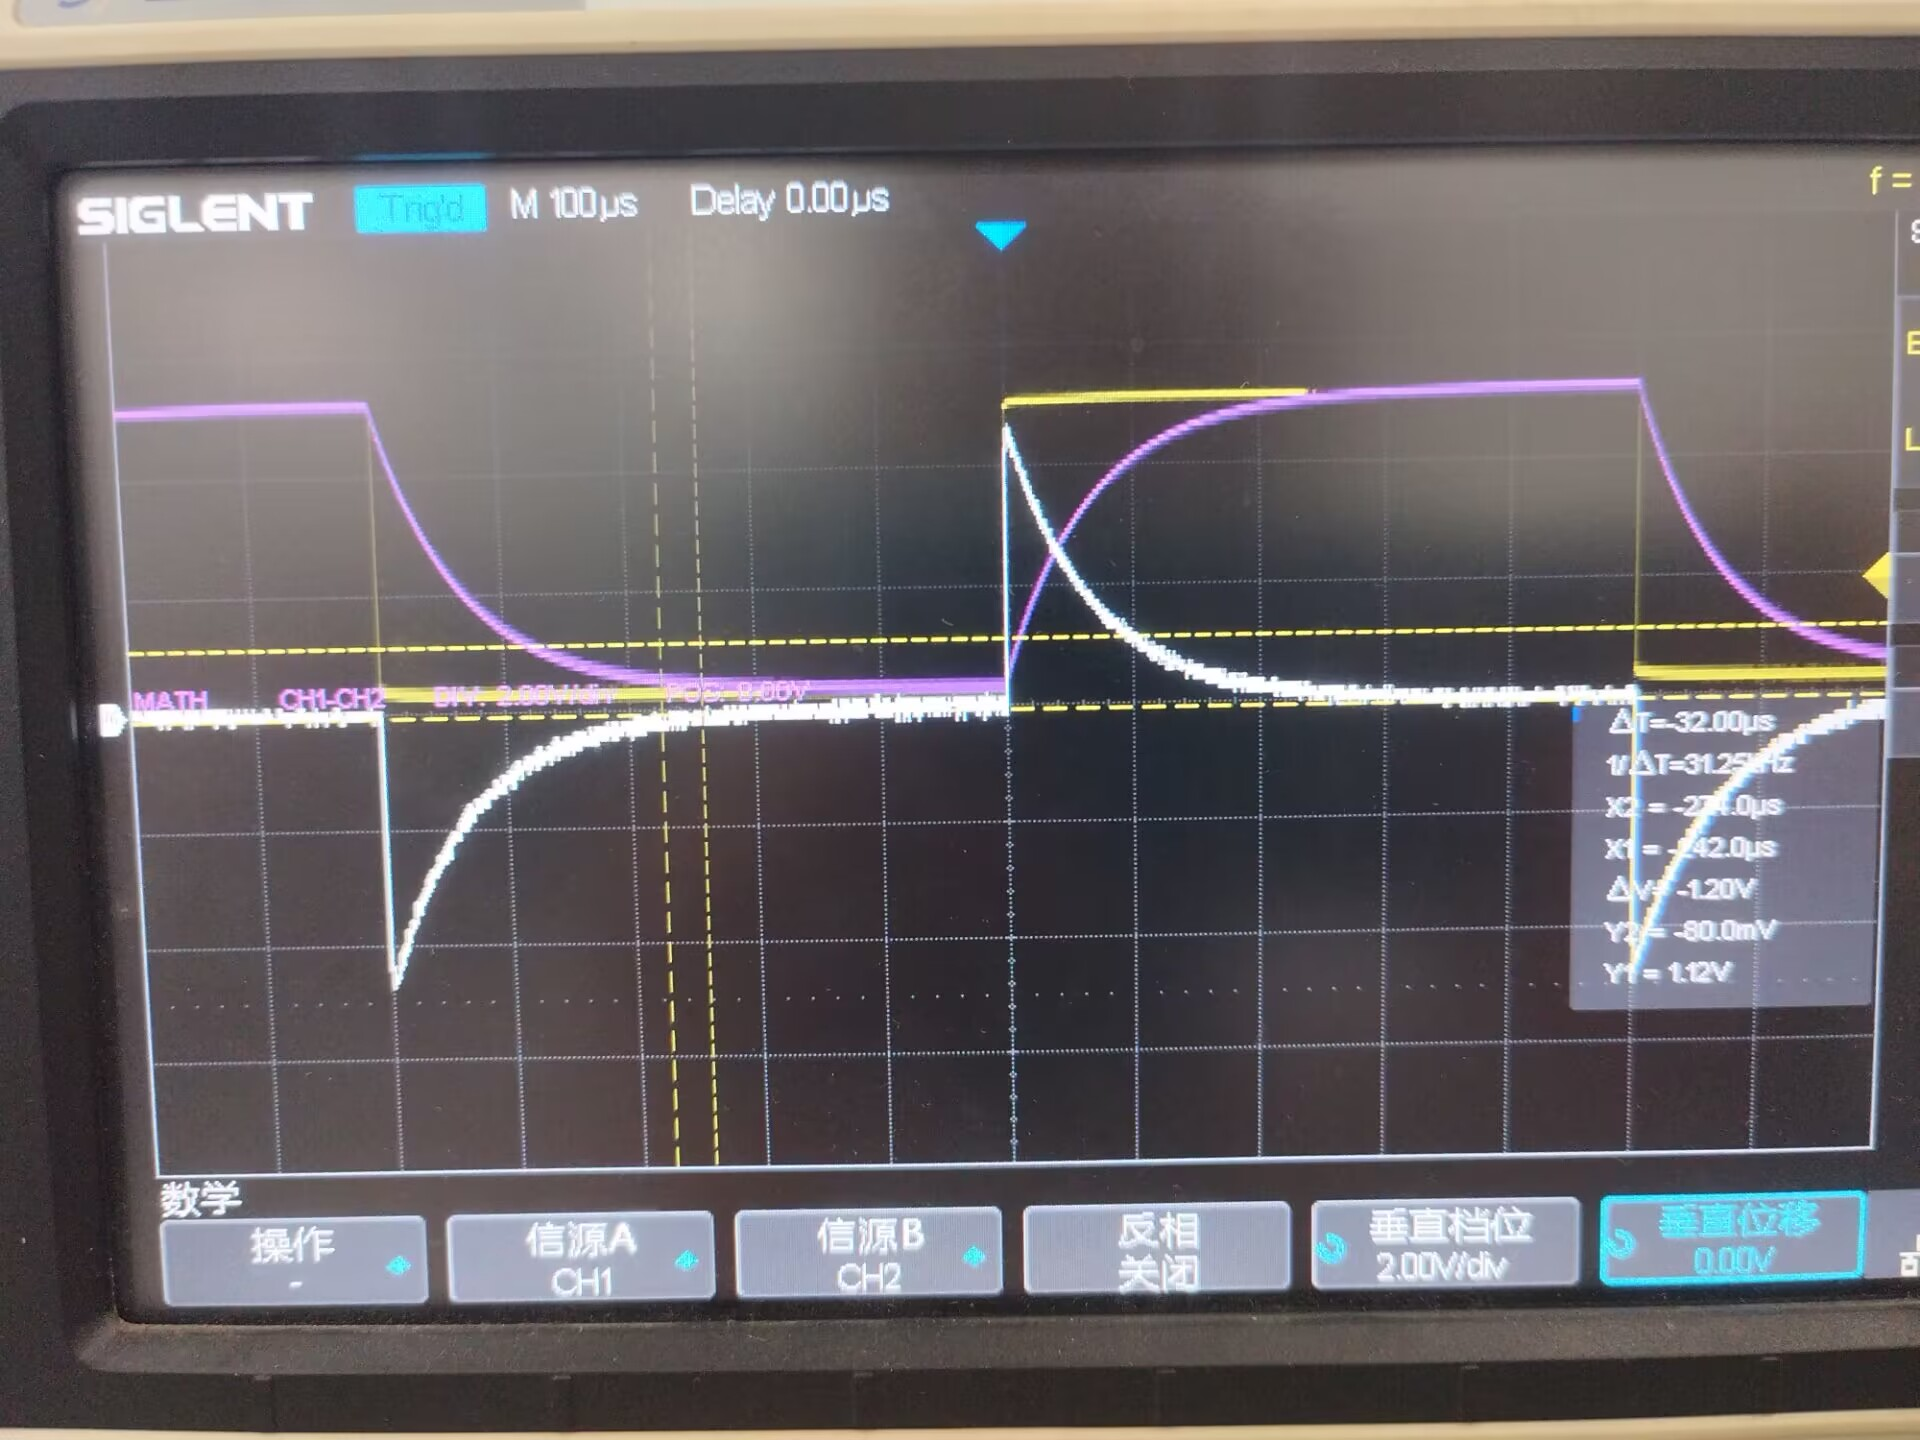
\includegraphics[scale=0.2]{pic/1_1.jpg}
    \caption{1-1}
    \label{fig:1-1}
\end{figure}
图中红色部分是电容上的输出电压,黄色部分是电源的方波波形。使用示波器的MATH功能,将两个值做减法,得到电阻上的输出电压,再根据欧姆定理可以得到回路的电流函数$i_C(t)$,如图中白色曲线所示。

可以看到$u_C(t)$按照指数规律衰减。这是由于方波输入可以分解为一系列的阶跃响应的叠加
\begin{equation}
    u_s(t)=u_s u(t)-u_s u(t-\dfrac{T}{2})+\dots
\end{equation}
而阶跃响应的公式为:
\begin{equation}
    u_C(t)=(u_C(0_{-})-U_s)e^{-\dfrac{t}{\tau}}+U_s
\end{equation}
所以输出电压$u_C(t)$可以表示为
\begin{equation}
    u_C(t)=
    \begin{cases}
        u_s(1-e^{-\dfrac{t}{\tau}}),0\leq t\leq \dfrac{T}{2}\\
        u_s e^{-\frac{t-\frac{T}{2}}{\tau}},\dfrac{T}{2}\leq t\leq T
    \end{cases}
\end{equation}
于是呈现出图示的波形。
\subsubsection{测出电路实际时间常数$\tau$。}
在示波器上通过光标测量(图\ref{fig:1-2}),得到波形上升到63.2\%所用的时间$\tau=66\mu$s,这与实验预期结果吻合很好。
\begin{figure}
    \centering
    \includegraphics[scale=0.1]{pic/1_2.jpg}
    \caption{1-2}
    \label{fig:1-2}
\end{figure}
\subsubsection{将 R 值增至 10 倍值,输入激励信号不变,观察响应$u_C(t)$波形现象做如何变化,并作记录分析。}
R增大至3$k\Omega$,电路图如图\ref{fig:实验1电路实物图}所示
\begin{figure}
    \centering
    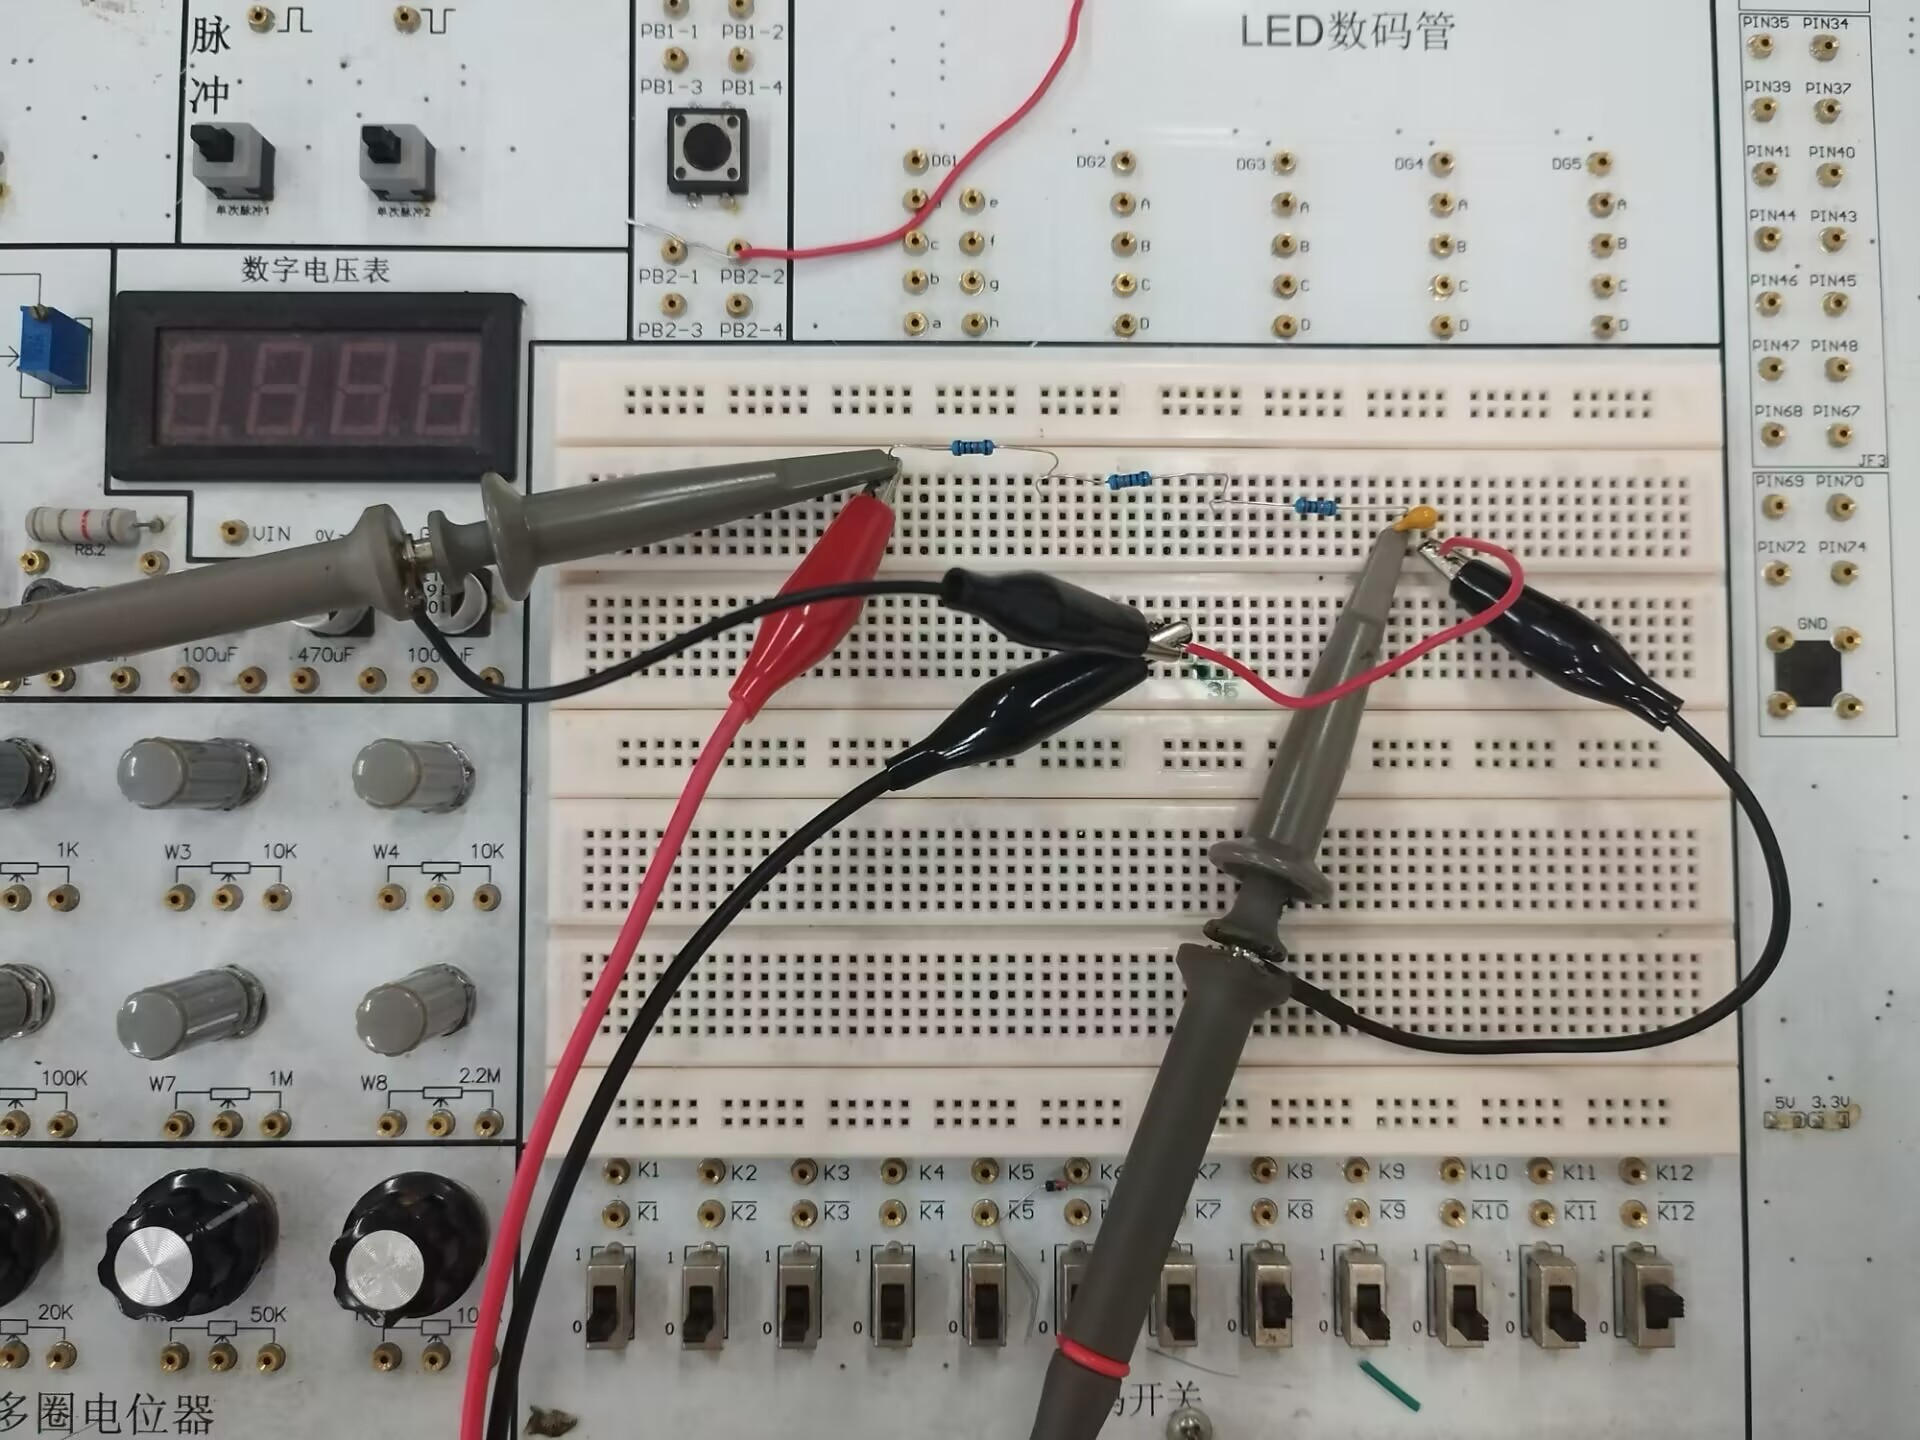
\includegraphics[scale=0.2]{pic/1_circuit.jpg}
    \caption{实验1电路实物图}
    \label{fig:实验1电路实物图}
\end{figure}
这时测得波形为图\ref{fig:1-3}。
\begin{figure}
    \centering
    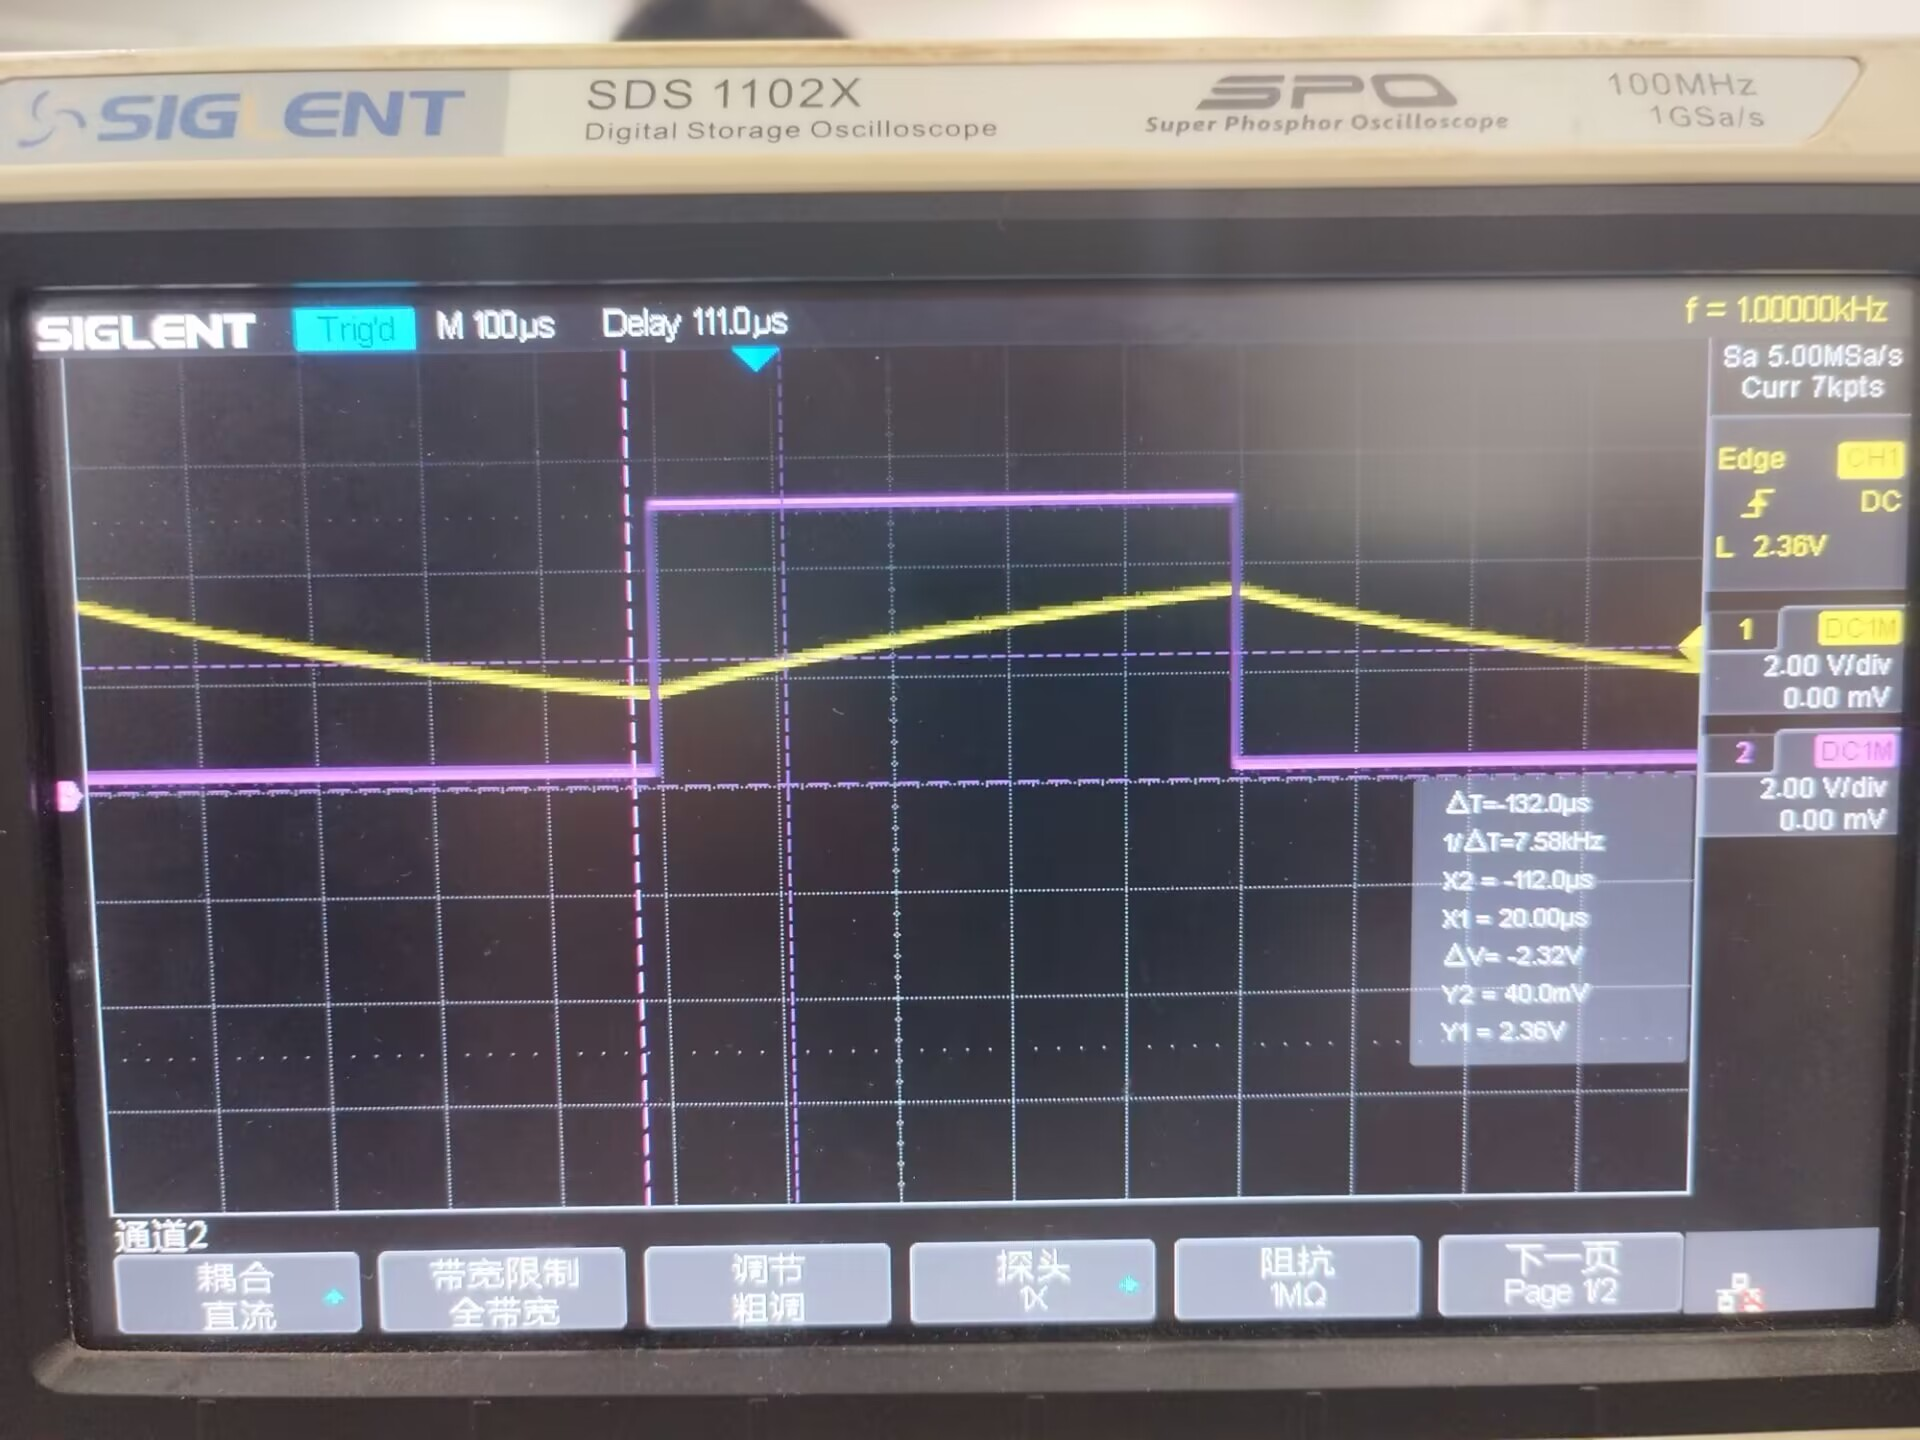
\includegraphics[scale=0.2]{pic/1_3.jpg}
    \caption{1-3}
    \label{fig:1-3}
\end{figure}
可以看到,在每个周期内,电容都不能充分地充放电,输出电压呈现近似三角波的形状。这是因为R提高后,时间常数增大,不能满足周期远大于时间常数的限制条件。
\subsubsection{要能保持(1)中响应$u_C(t)$波形现象,如何调整输入信号?观察记录调整后的$u_C(t)$波形。}
为此,通过调小电源的频率,增大方波的周期,使得在一个周期内,电容能够完整地充电,从而获得完整的充电波形。当电源频率减小到52Hz时,电容可以很充分地充放电,如图\ref{fig:1-4}所示。
\begin{figure}
    \centering
    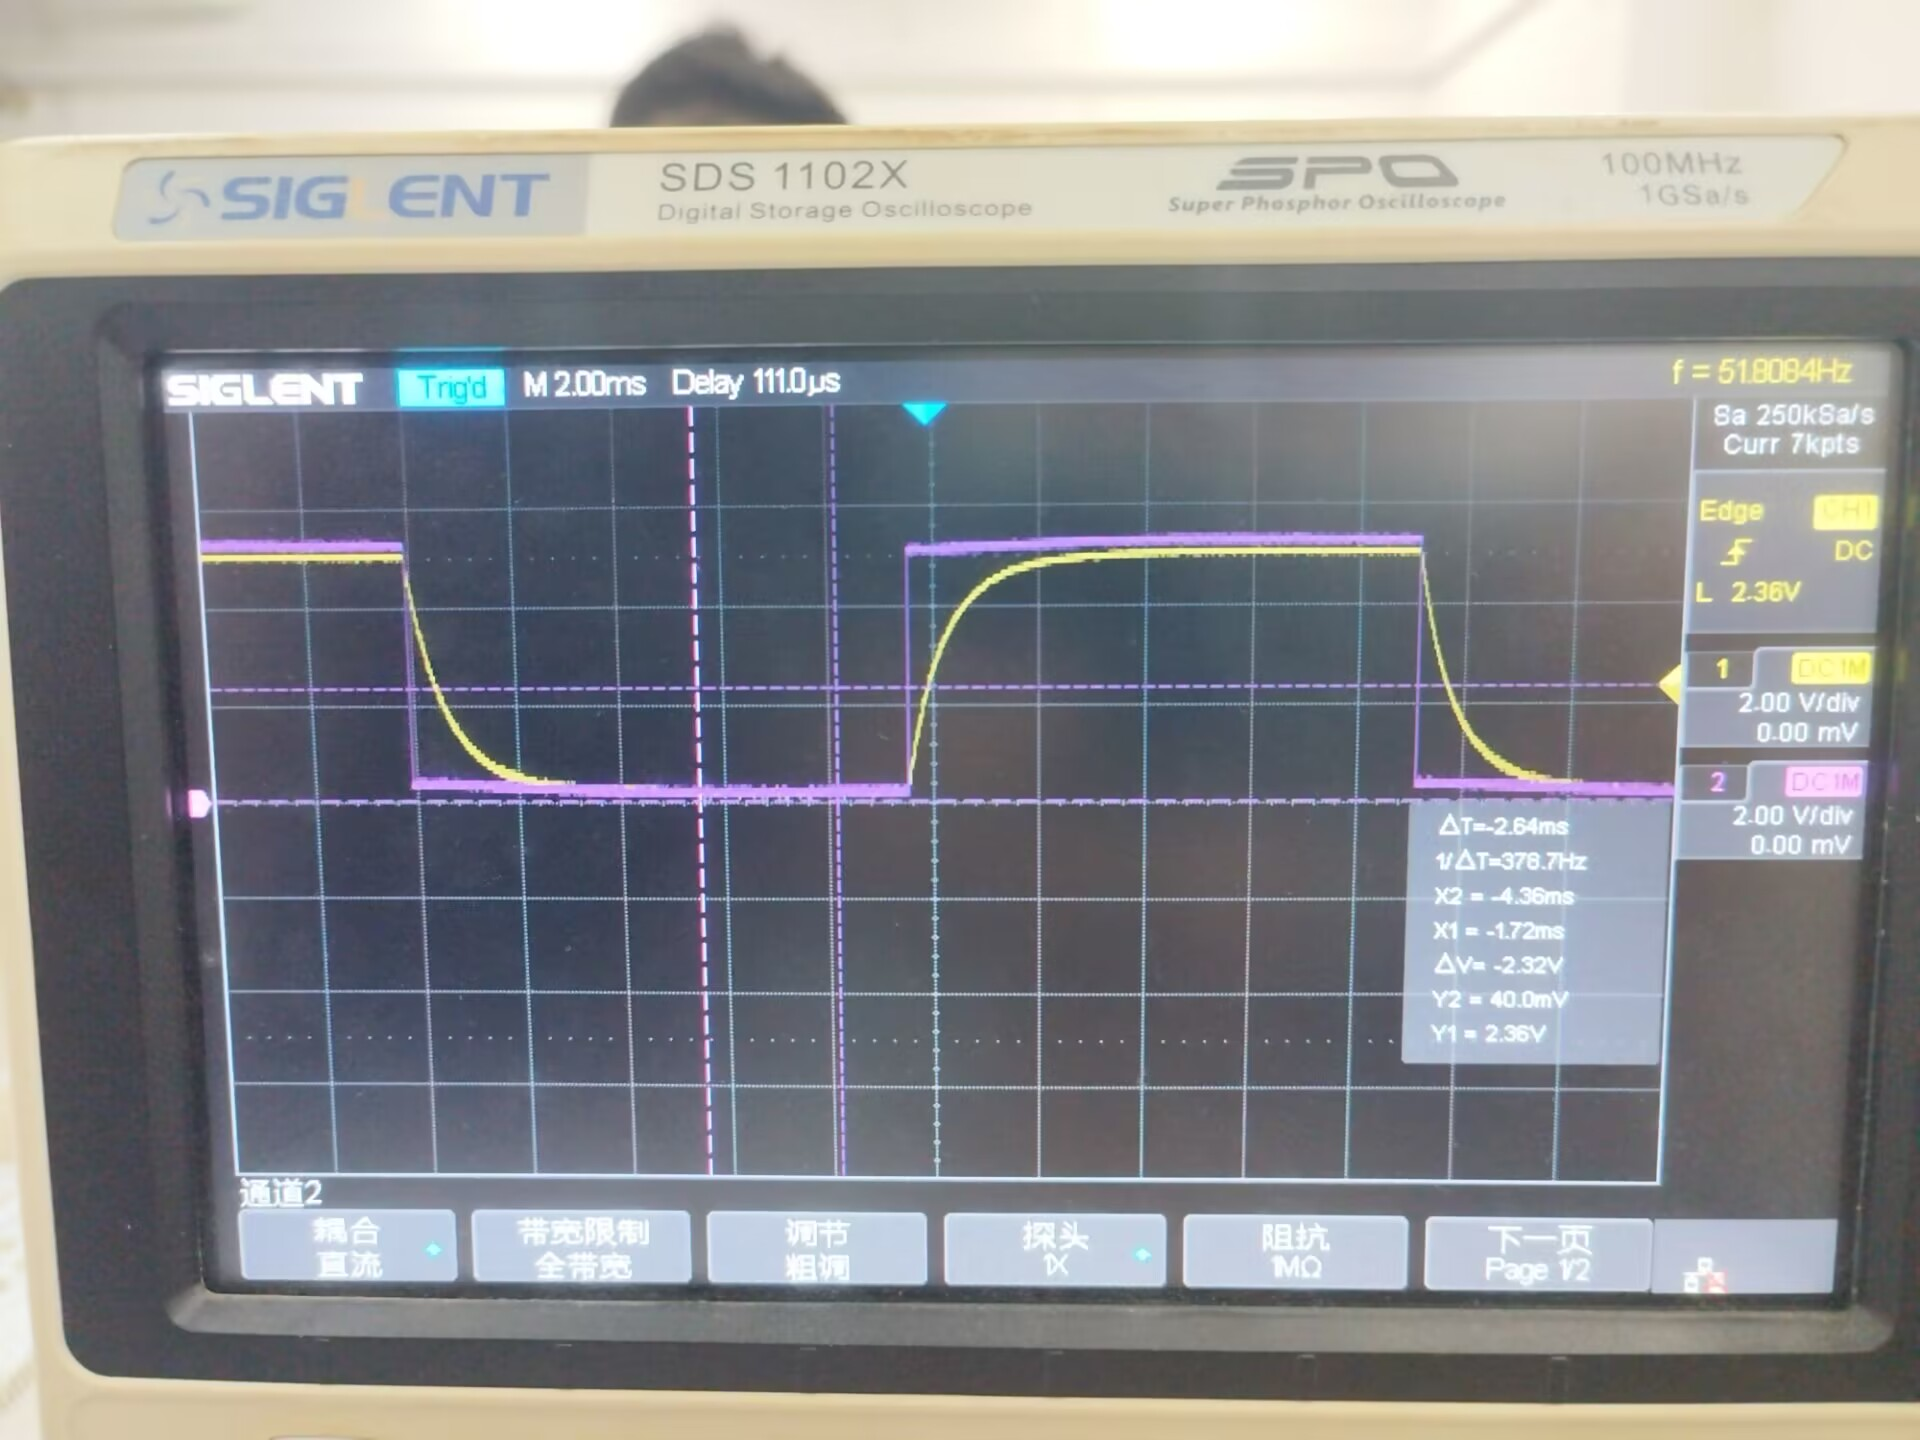
\includegraphics[scale=0.2]{pic/1_4.jpg}
    \caption{1-4}
    \label{fig:1-4}
\end{figure}

\subsection{积分电路}
\subsubsection{电路参数选取}
根据上文实验原理的分析,要想保持时间常数$\tau=0.22ms$,结合现有的电容$C=22dF$,得到应选择一个阻值为$10k\Omega$的电阻。
为了满足$\tau > 5T$的要求,设置电路频率为22727Hz。
\subsubsection{电路实物图}
积分电路的连接如图\ref{fig:积分电路实物图}所示
\begin{figure}[h]
    \centering
    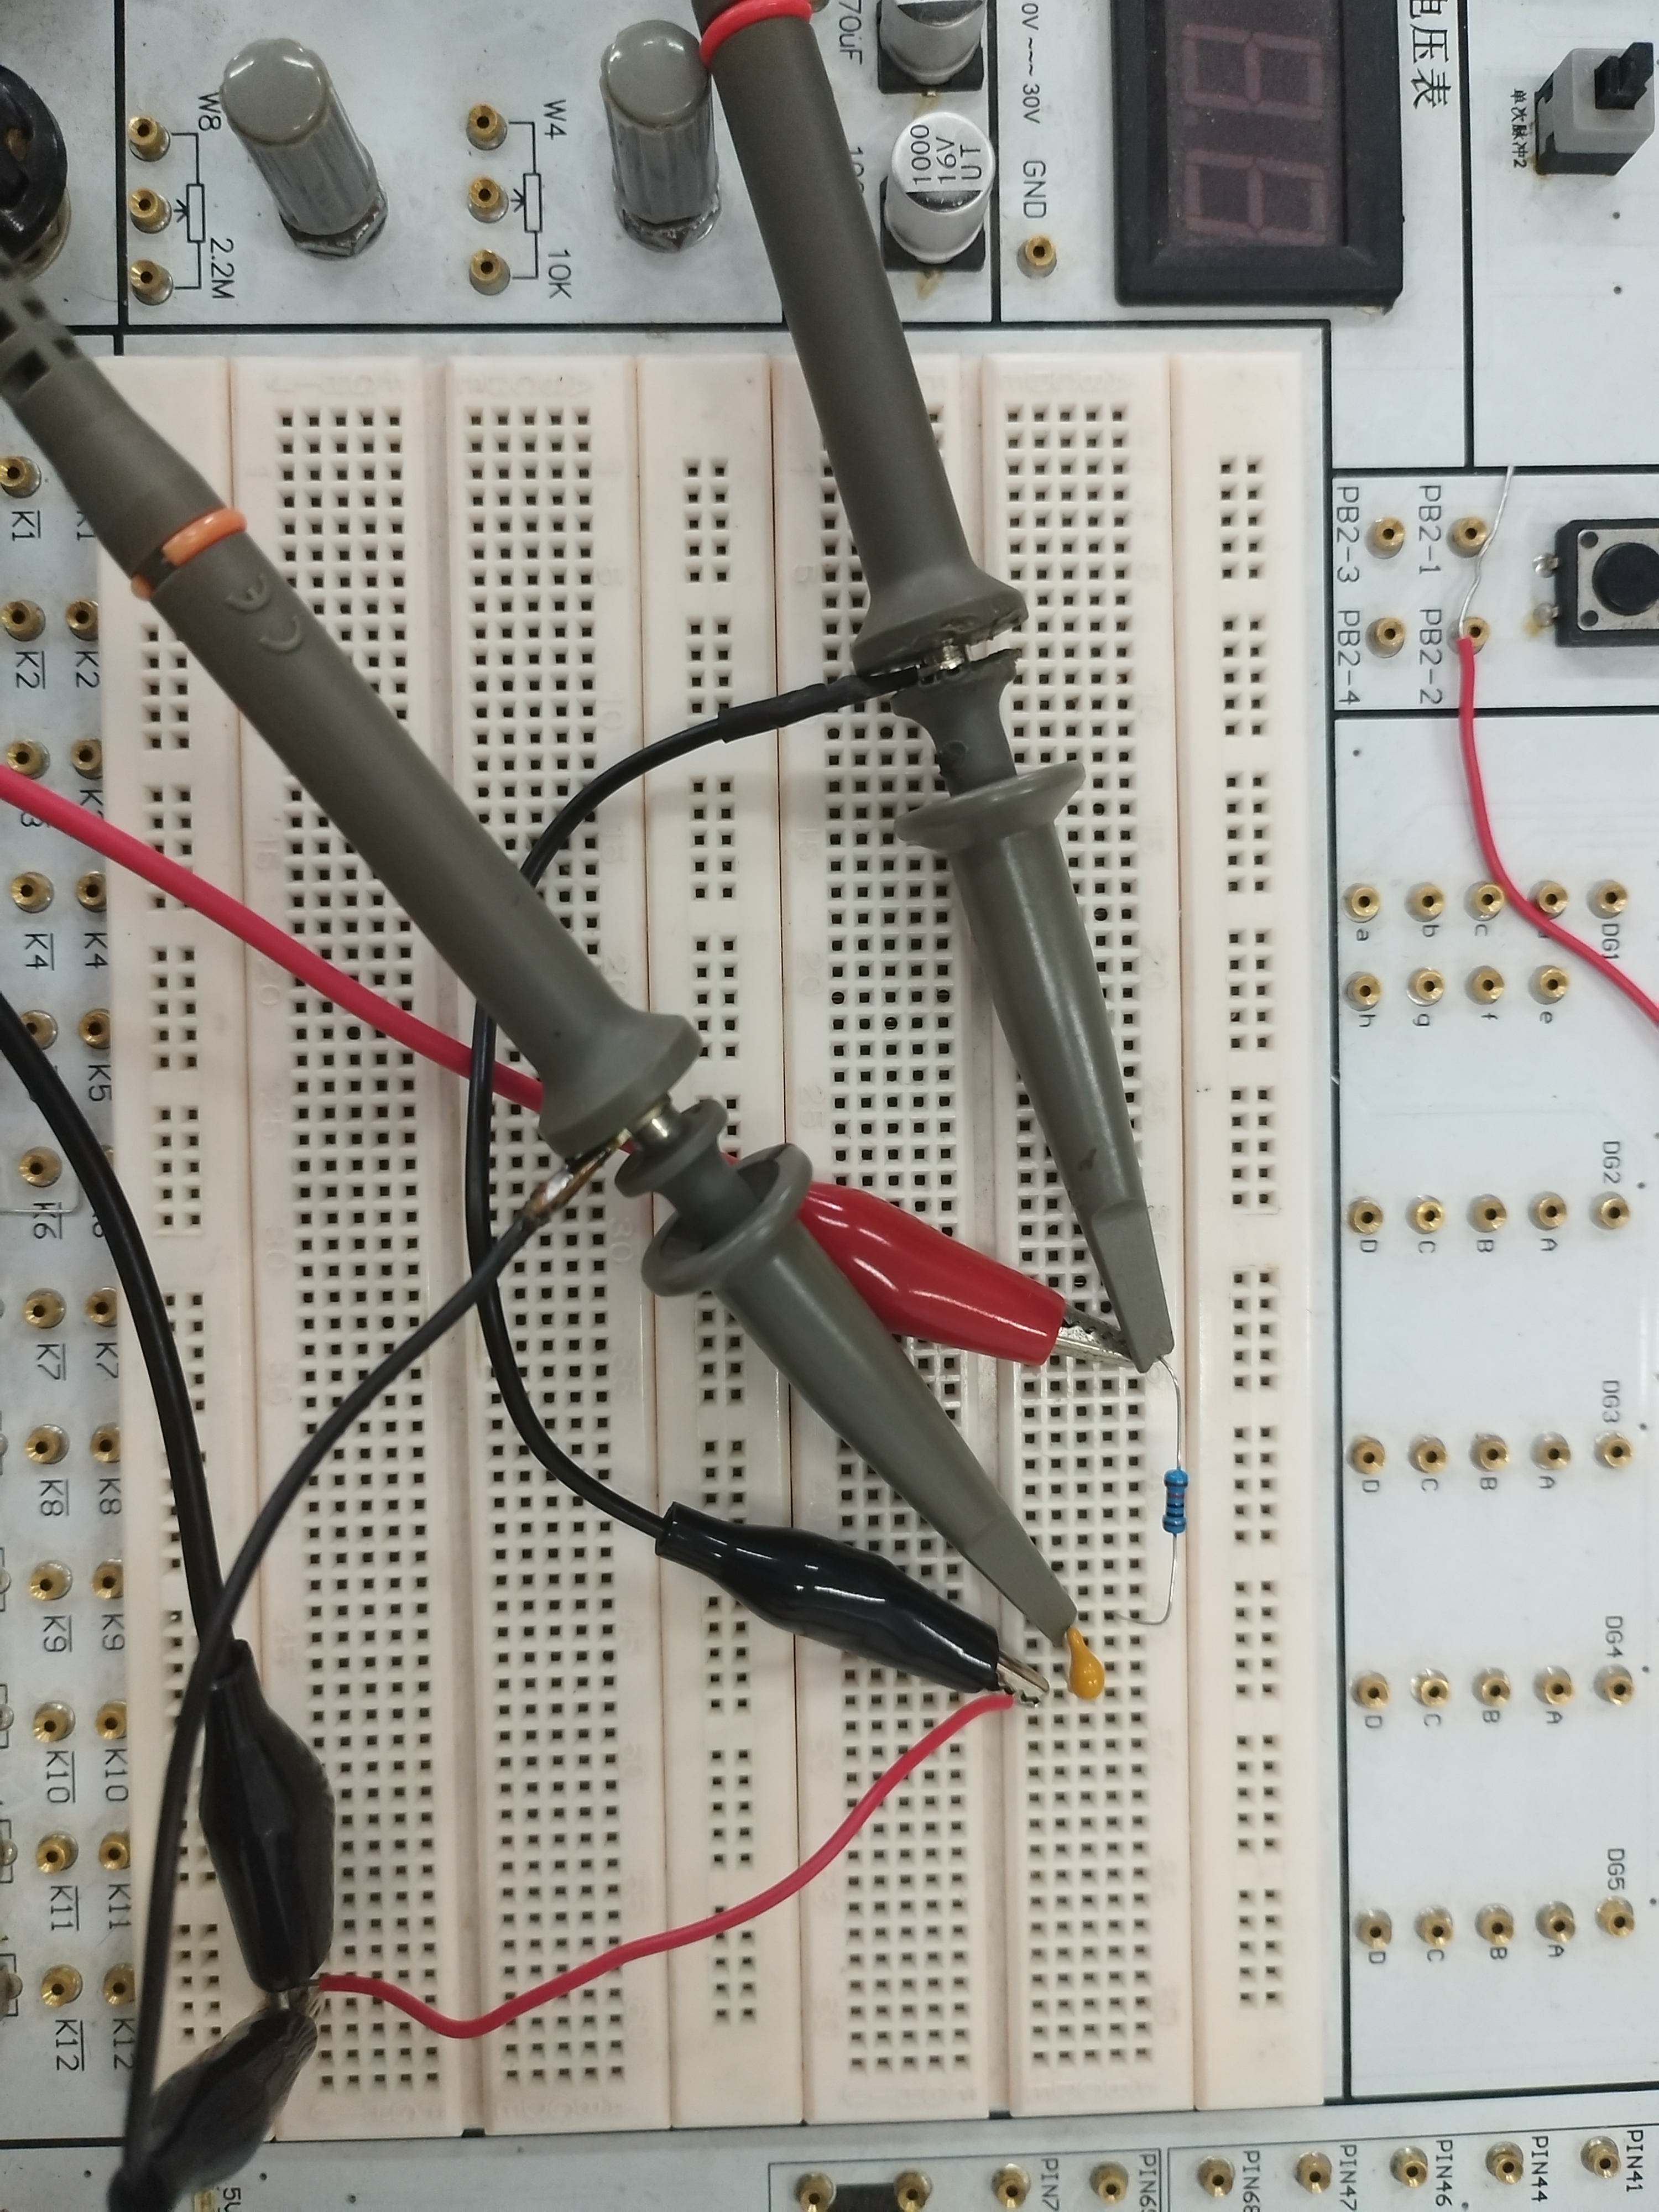
\includegraphics[scale=0.08]{pic/int_cir.jpg}
    \caption{积分电路实物图}
    \label{fig:积分电路实物图}
\end{figure}
\subsubsection{结果与分析}
采用光标方法测量,测得输出电压$u_C$的Top=135mV,Base=-134mV,即$\Delta u_O$=Pk-Pk=269mV。电源$U_s$的Top=5.04V,Base=240mV。与Multisim仿真结果$\Delta u_O= 247.188mV$比较,误差在8\%左右,可以接受。
\subsection{微分电路}
\subsubsection{电路参数选取}
电容和电阻的参数保持不变,要想满足$\tau < 0.05T$的要求,设置电路频率为227.27Hz。
\subsubsection{电路实物图}
微分电路的连接如图\ref{fig:微分电路实物图}所示
\begin{figure}[!ht]
    \centering
    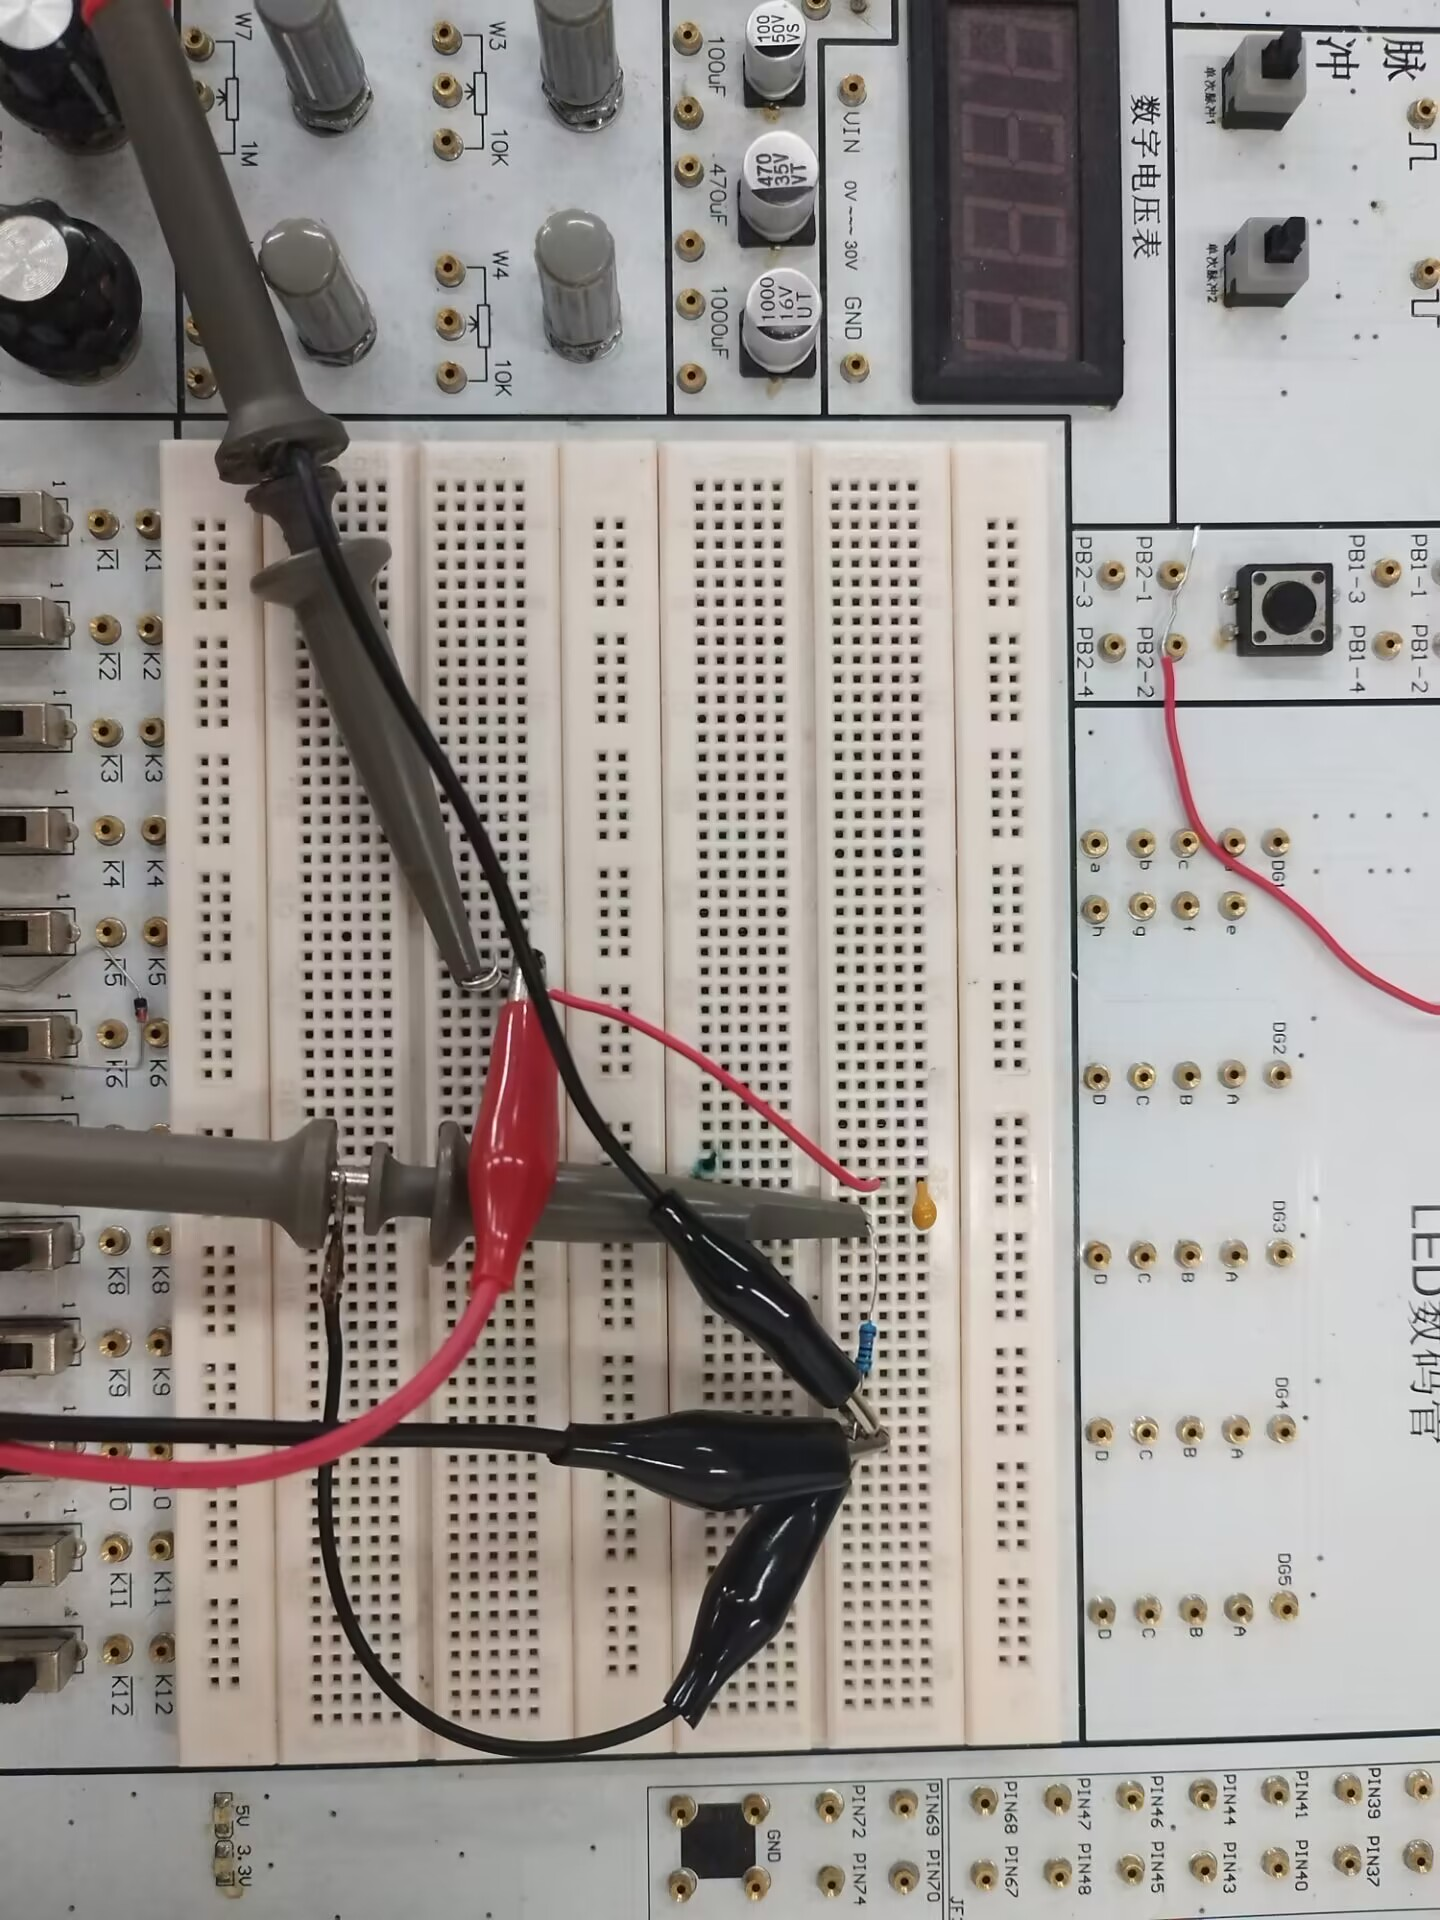
\includegraphics[scale=0.2]{pic/dif_cir.jpg}
    \caption{微分电路实物图}
    \label{fig:微分电路实物图}
\end{figure}
\subsubsection{结果与分析}
采用光标方法测量,测得输出电压$u_C$的Top=5.08V,Base=-4.64V,即$\Delta u_O$=Pk-Pk=9.72V。电源$U_s$的Top=5.04V,Base=240mV。与Multisim仿真结果$\Delta u_O= 9.865V$比较,误差在1.5\%左右,可以接受。
\section{实验仪器}
\begin{enumerate}
    \item 鼎阳SDS1000X
    \item 万用表UT803
    \item 信号源SDG1000X
\end{enumerate}
\section{实验总结}
本次实验研究了RC电路的方波响应,设计了积分和微分电路。实验效果总体较好,但是出现了两个问题。一是数据记录没有条理性,导致在测量过程中出现了实验照片忘拍的情况,需要重新搭建电路来实验,拖慢实验进度。二是对示波器的操作问题。在测量积分电路的$\Delta u_O$时,最开始直接使用Measure方法。由于波形本身在顶点处有较大波动,导致测量值明显偏离正常误差范围。最后通过手动调节光标得到了合理的测量值。
\section{参考文献}
无

\end{document}
